\famichapter{Authentication, Authorization, and Security}{This chapter explains
how FamiPet establishes user identity, how it enforces authorization, and the
security controls applied at the HTTP and storage layers.}{ch:auth}

\section{Content}
\label{sec:authoverview}

Authentication is handled entirely by the backend. The flow has three stages:
account creation with e-mail verification, login with a signed token, and
token-based access control for every protected route. Figures~\ref{fig:reg}
through~\ref{fig:reset} show the four authentication workflows as implemented.

\subsection{Registration and E-mail Verification}

\begin{figure}[htbp]
    \centering
    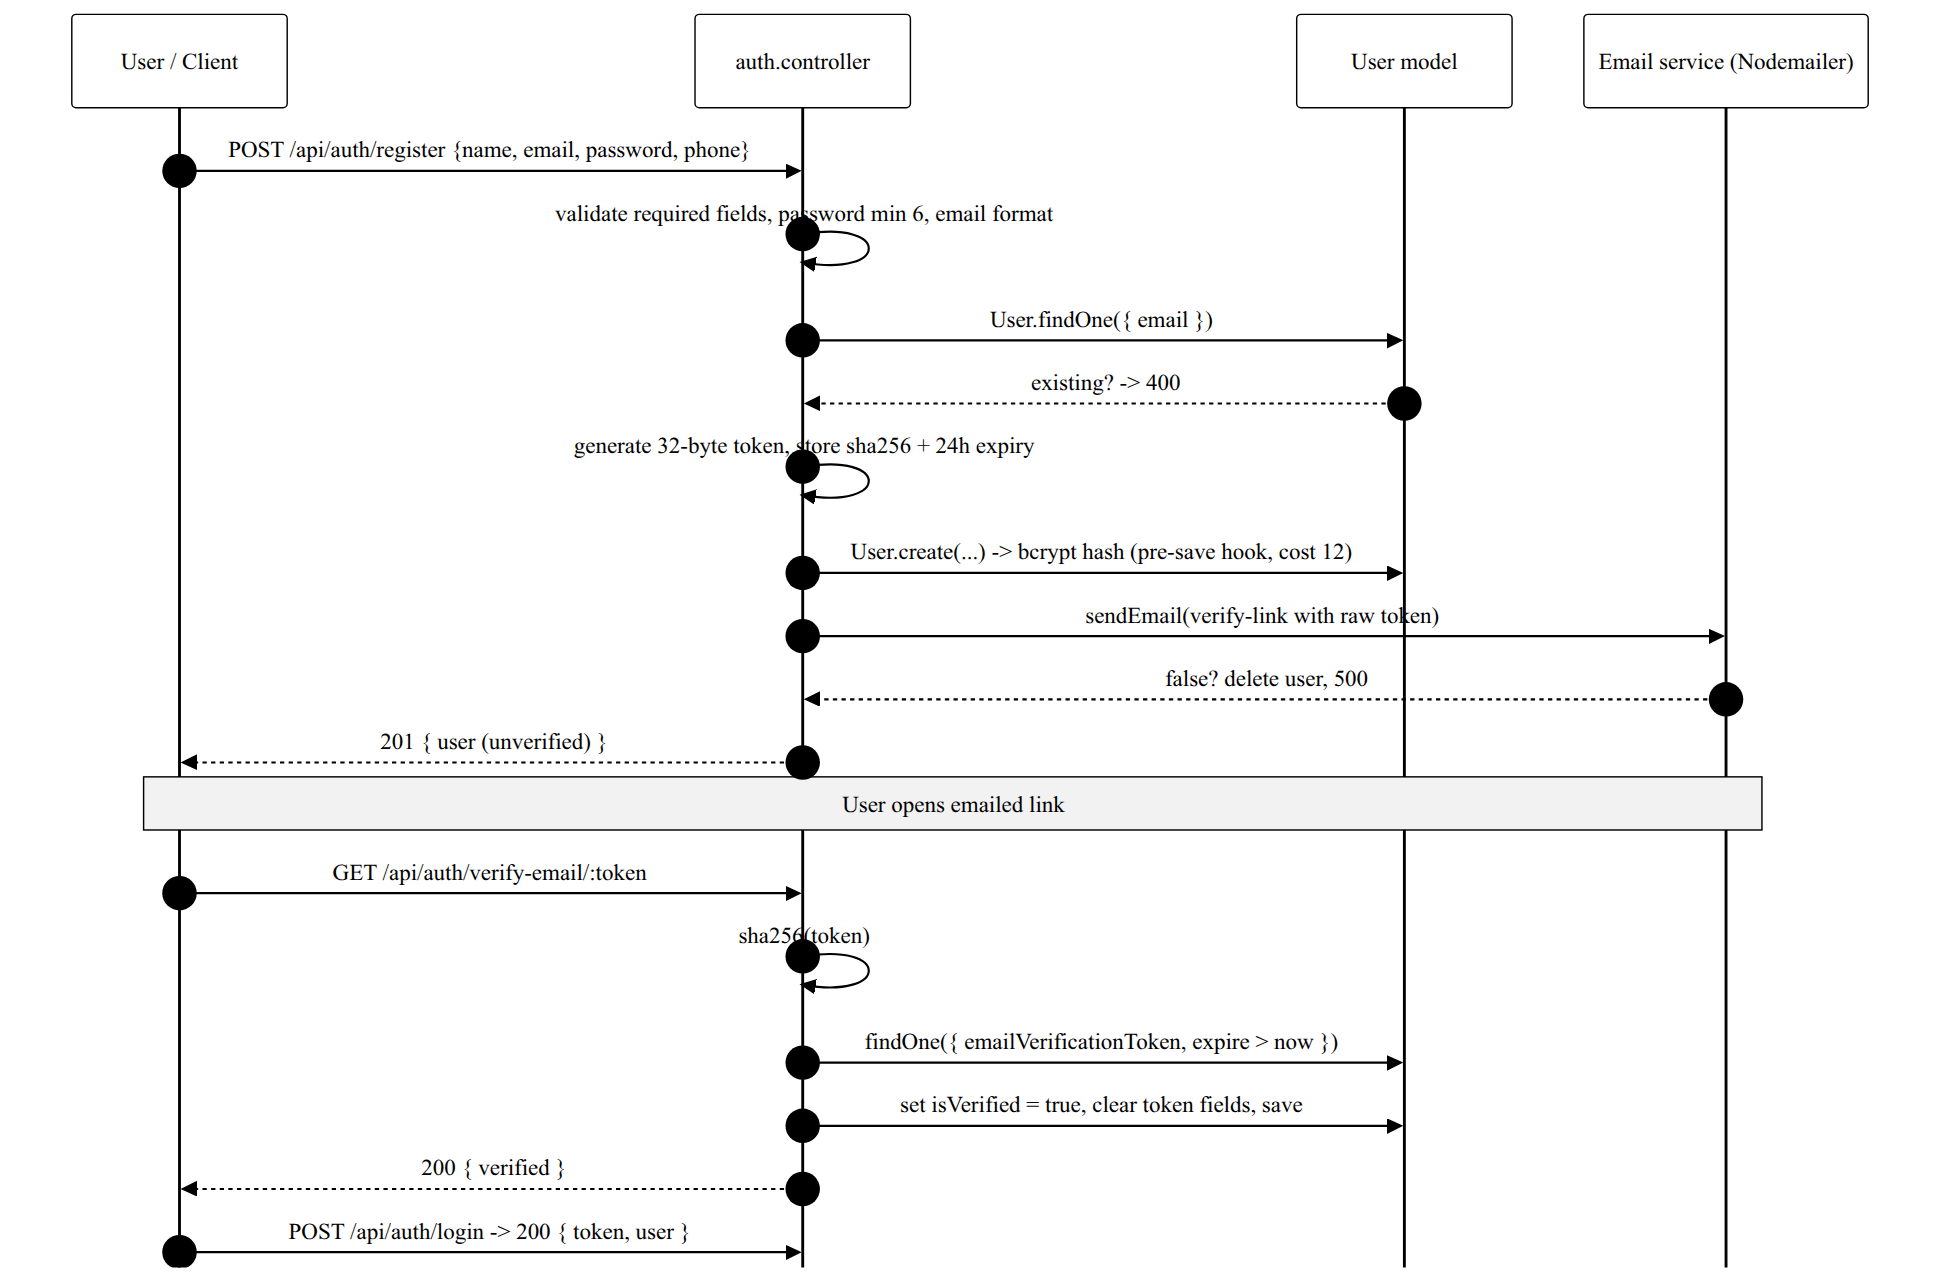
\includegraphics[width=\textwidth]{figures/09-register-verify.png}
    \caption{Registration and e-mail verification flow.}
    \label{fig:reg}
\end{figure}

When \texttt{POST /api/auth/register} is received, the controller validates the
fields, normalizes the e-mail, checks whether it already exists, generates a
32-byte verification token, stores only its SHA-256 hash with a 24-hour expiry,
hashes the password through the pre-save hook, and creates the user with
\texttt{isVerified: false}. An HTML e-mail containing a verification link is
sent through Nodemailer; if the e-mail cannot be sent the user document is
deleted so no unverifiable account remains. Clicking the link calls
\texttt{GET /api/auth/verify-email/:token}, which hashes the presented token and
marks the user verified. A resend endpoint generates a fresh token for
unverified accounts. Login is refused for unverified accounts
(HTTP 403, \texttt{isVerified: false} in the response).

\subsection{Login and Token Issuance}

\begin{figure}[htbp]
    \centering
    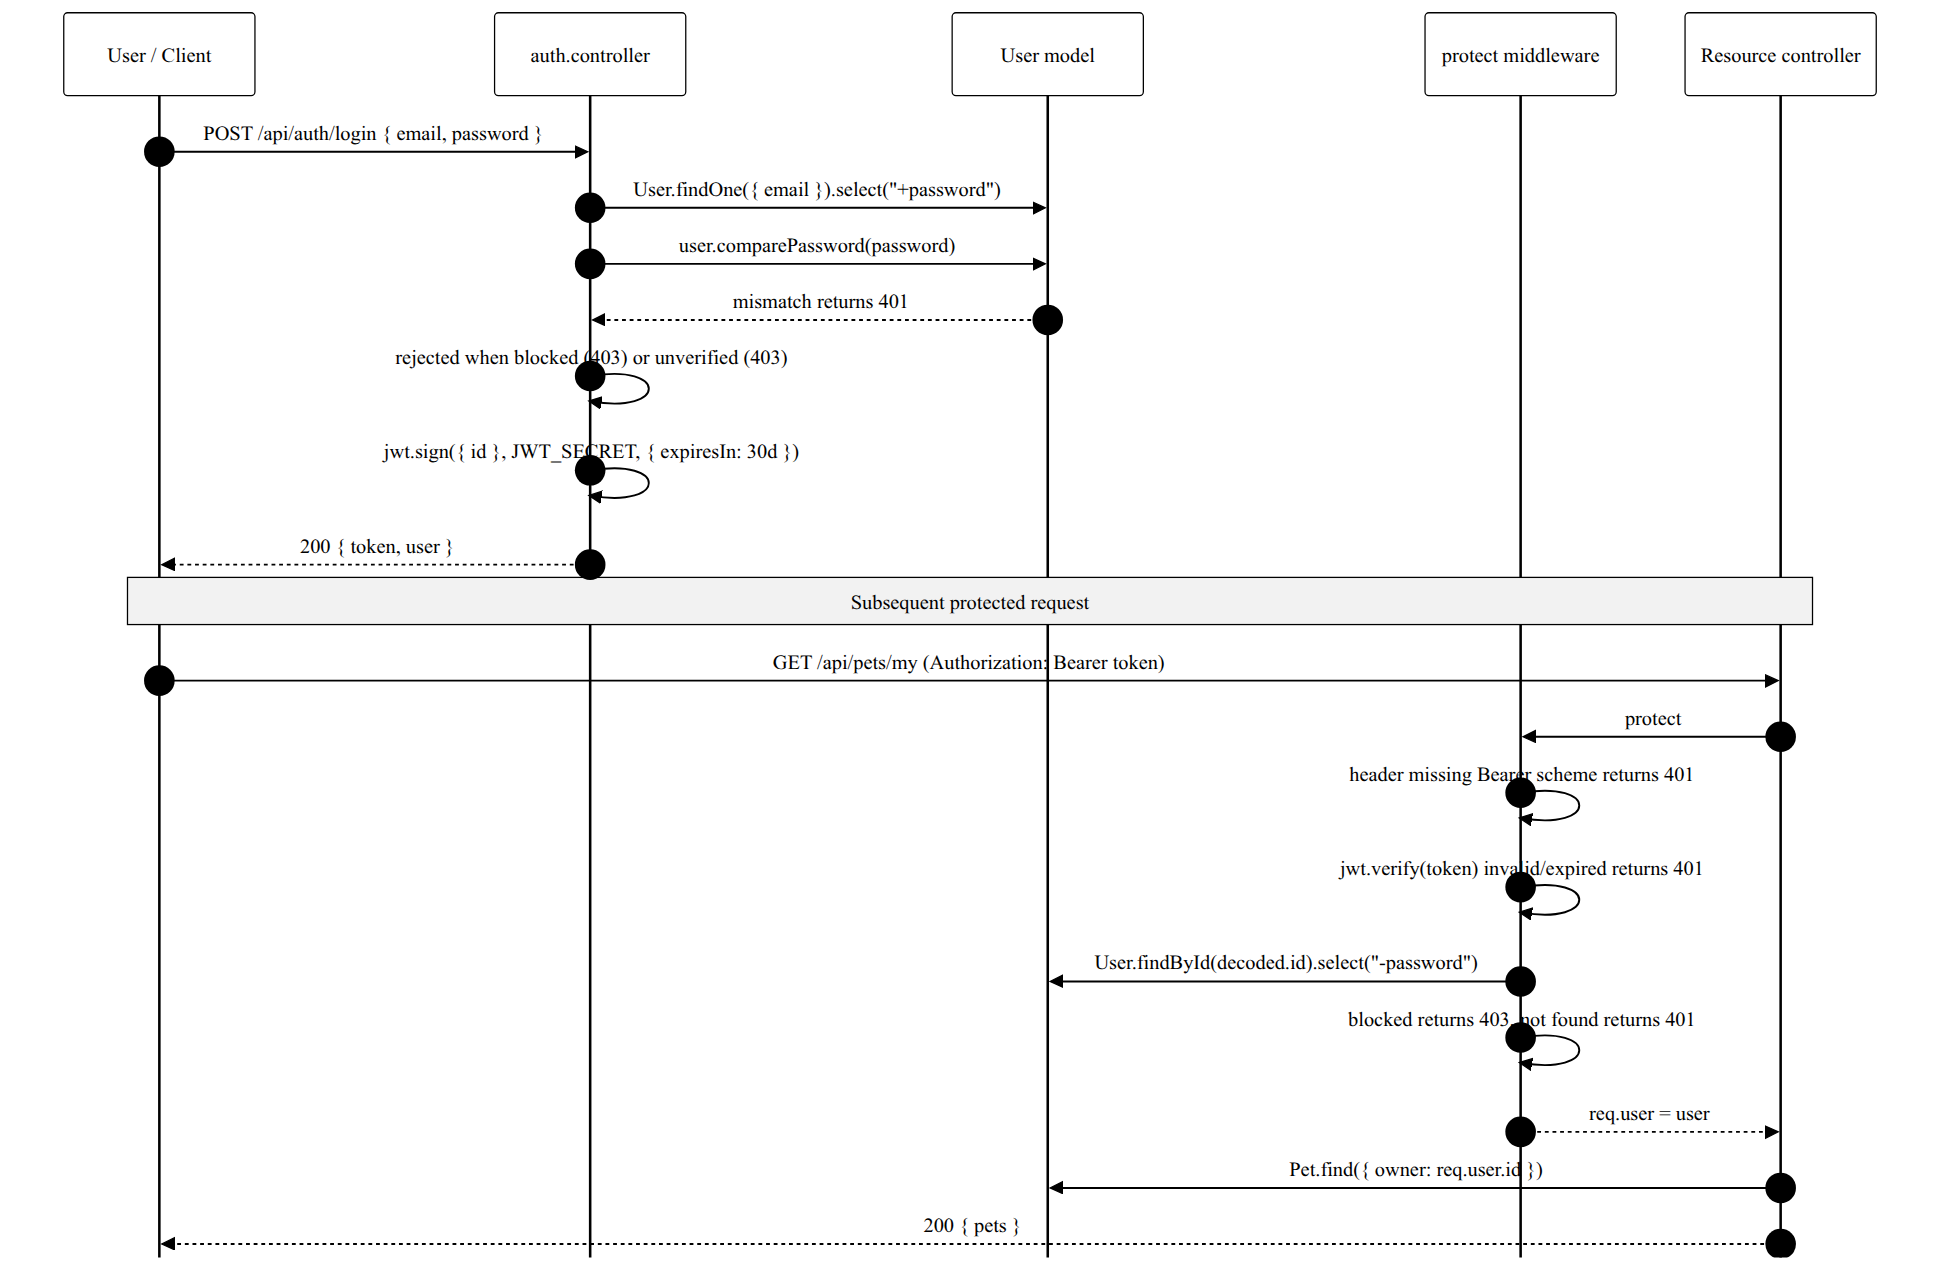
\includegraphics[width=\textwidth]{figures/10-login-token.png}
    \caption{Login and JWT issuance flow.}
    \label{fig:login}
\end{figure}

\texttt{POST /api/auth/login} selects the user including the (normally excluded)
password, compares the presented password with the stored bcrypt hash, refuses
blocked and unverified accounts, and on success signs a JWT containing the user
identifier with the configured secret and a 30-day expiry (\texttt{JWT\_EXPIRE}).
The client stores the token and sends it as a bearer header on protected calls.
The \texttt{/api/auth/me} endpoint returns the current user with pets and
favourites populated.

\subsection{Token Verification and Role-Based Access}

Every protected route is wrapped by the \texttt{protect} middleware
(\texttt{backend/middleware/auth.js}). Figure~\ref{fig:access} shows its decision
tree.

\begin{figure}[htbp]
    \centering
    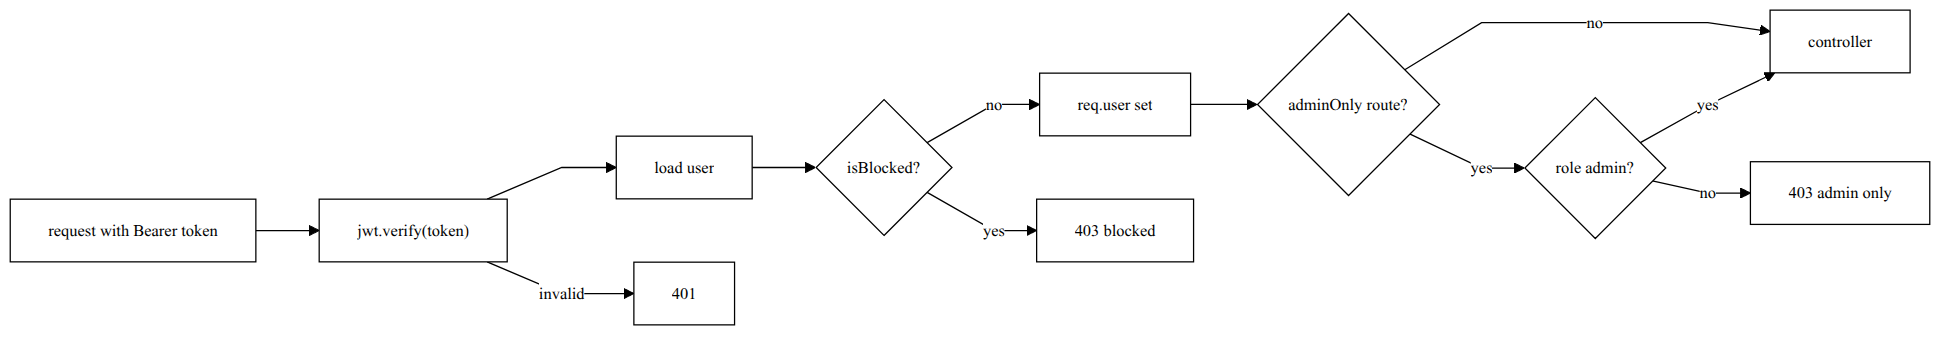
\includegraphics[width=\textwidth]{figures/11-access-control.png}
    \caption{Access-control decision tree (protect and adminOnly).}
    \label{fig:access}
\end{figure}

The middleware rejects requests without a bearer header (401), without a
configured \texttt{JWT\_SECRET} (500), with an invalid token (401), with a
missing user (401), or with a blocked account (403). On success it assigns
\texttt{req.user} from the database (excluding the password) and forwards the
request. The \texttt{adminOnly} middleware then enforces
\texttt{req.user.role === "admin"} for administrative routes, returning 403
otherwise. Ownership is applied separately inside the controllers: resources are
queried with the owner predicate and therefore return 404 for other users'
resources.

\subsection{Password Recovery}

\begin{figure}[htbp]
    \centering
    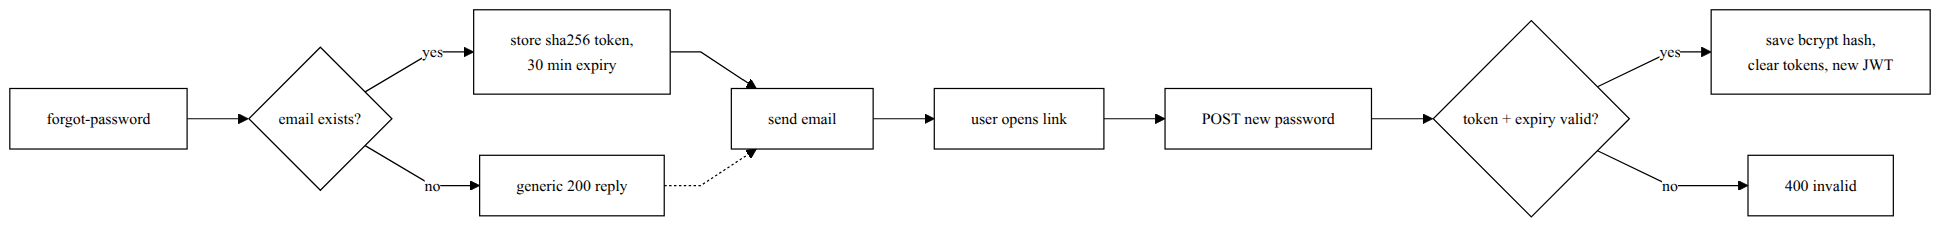
\includegraphics[width=\textwidth]{figures/12-password-reset.png}
    \caption{Password reset flow.}
    \label{fig:reset}
\end{figure}

\texttt{POST /api/auth/forgot-password} always returns a generic ``if the e-mail
is registered'' message so that the endpoint cannot be used to enumerate
accounts. A registered e-mail receives a link containing a 32-byte token; the
server stores only the SHA-256 hash with a 30-minute expiry. \texttt{POST
/api/auth/reset-password/:token} hashes the presented token, verifies it and the
expiry, stores the new password (bcrypt-hashed by the pre-save hook), clears the
token fields, and returns a fresh JWT so the user is logged in immediately. If
the e-mail cannot be delivered the stored token is cleared so a stale, unusable
token is not left on the account. A separate \texttt{change-password} endpoint
requires the current password.

\section{Security Controls}
\label{sec:security}

The security controls below are implemented and were verified in the Step 10
test campaign (Chapter~\ref{ch:testing}).

\begin{center}
\begin{longtable}{@{}p{3.6cm}p{11.0cm}@{}}
\toprule
\textbf{Control} & \textbf{Implementation} \\
\midrule
Password hashing & bcrypt cost 12 (\texttt{\$2a\$12\$} hashes verified directly
in the database). \\
Token hygiene & Verification and reset tokens are stored hashed (SHA-256);
plaintext tokens appear only in e-mail links. \\
JWT & Signed bearer tokens with \texttt{JWT\_SECRET}; invalid or expired tokens
yield 401. \\
E-mail verification gate & Unverified accounts cannot log in; forgot-password
does not reveal whether an e-mail exists. \\
Ownership isolation & All user-scoped queries bind to \texttt{req.user.\_id};
cross-user access to appointments, reminders, notifications, health records, and
vaccinations returns 404. \\
Role enforcement & \texttt{adminOnly} on all administrative routes; a regular
user receives 403. \\
Input validation & Backend-side checks for required fields, e-mail format,
password length, valid ObjectIds, real dates, ownership, and state transitions
returning 400/404/500. \\
CORS & Origin guard accepting the configured client, localhost, and private LAN
origins; preflight OPTIONS answered 204. \\
Security headers & Helmet headers with \texttt{crossOriginResourcePolicy:
cross-origin} so uploaded images are embeddable by the frontend origin. \\
Secret management & Keys live only in \texttt{backend/.env} (git-ignored);
only placeholder \texttt{.env.example} is committed; no secrets in repository
history. \\
Blocked accounts & \texttt{protect} and \texttt{login} reject blocked users with
403. \\
\bottomrule
\end{longtable}
\end{center}

\section{Security Boundary Verification}

The boundary behaviour was tested with two identities: a regular user and an
administrator. A regular user calling nine administrative endpoints
(\texttt{/api/admin/dashboard}, \texttt{/api/admin/users}, \texttt{/api/admin/
pets}, adoption listing and status update, \texttt{DELETE /api/admin/users/:id},
breed and veterinarian creation, and lost-and-found moderation) received 403 on
every call. A user attempting to read, update, or cancel another user's
appointment received 404 because the query is owner-scoped. These results are
recorded in the testing chapter (Chapter~\ref{ch:testing}).